\documentclass[10pt, a4paper]{article}

\usepackage[utf8]{inputenc}
\usepackage[T1]{fontenc}
\usepackage[english]{babel}
\usepackage{amsmath, amssymb, amsthm}
\usepackage{graphicx}
\usepackage{geometry}
\usepackage{hyperref}
\usepackage{xurl}
\usepackage{cite}
\usepackage{booktabs}
\usepackage[nopatch=footnote]{microtype}
\usepackage{setspace}
\usepackage{titlesec}
\usepackage{lmodern}
\usepackage{enumitem}
\usepackage{array}

\geometry{margin=2.5cm}
\setlength{\columnsep}{0.7cm}
\setstretch{1.08}
\emergencystretch=1.2em
\setlength{\parskip}{0.35em}
\setlength{\parindent}{0pt}

\hypersetup{
    colorlinks=true,
    linkcolor=black,
    citecolor=black,
    urlcolor=blue,
    pdftitle={Underdetermination of Finite Sequences and Construct Validity in Intelligence Testing},
    pdfauthor={[Roberto Ferrari]},
}

\theoremstyle{plain}
\newtheorem{theorem}{Theorem}
\newtheorem{proposition}{Proposition}
\newtheorem{corollary}{Corollary}
\theoremstyle{definition}
\newtheorem{definition}{Definition}
\theoremstyle{remark}
\newtheorem{remark}{Remark}

\titleformat{\section}{\large\bfseries}{\thesection.}{0.5em}{}
\titleformat{\subsection}{\normalsize\bfseries}{\thesubsection.}{0.5em}{}

\title{\textbf{Underdetermination of Finite Sequences and Construct Validity in Intelligence Testing:\\
an Accurate and Accessible Discussion of Interpolation, the $g$ Factor, and Numerical Completion Items}}

\author{
    [Roberto Ferrari]\\
    \small \texttt{[robertoferrari966@gmail.com]}
}

\date{\today}

\begin{document}

\maketitle
\thispagestyle{empty}

\begin{abstract}
Numerical sequence completion items are among the most familiar tasks in
reasoning tests: a respondent is shown a finite set of terms and asked to state
the next one. This article develops a precise claim, formulated in a way that
remains accessible while preserving mathematical rigor: \emph{given only the
observed terms, the next term is not uniquely determined as a matter of logic
unless additional assumptions are imposed on the class of admissible rules or on
the criterion used to select a rule}. The argument is established through
Lagrange interpolation and the explicit construction of infinite families of
functions compatible with the same data.

The second part of the paper addresses the psychometric question. It explains
what the $g$ factor is, why it was introduced in the intelligence literature,
how it is estimated through factor analysis, and in what sense it differs both
from a simple IQ score and from an ``essence'' directly observable in a person.
Conceptually, the central point is the following: the psychometric usefulness of
an item does not automatically eliminate the problem of how that item should be
interpreted. An item may correlate with other tests, contribute to the estimate
of $g$, and even have predictive value, while still being conceptually narrower
than ordinary language may suggest.

The conclusion is cautious but firm. Sequence items may measure real and useful
abilities, such as inferring the rule \emph{intended} by the test designer,
rapidly recognizing conventional regularities, and reasoning under time
constraints. However, without explicit constraints on the space of admissible
solutions, such items do not by themselves justify the claim that one specific
continuation is the only mathematically correct answer. For this reason, their
interpretation as a direct measure of ``general intelligence'' requires more
theoretical care than is often made explicit.
\end{abstract}

\vspace{1em}
\noindent\textbf{Keywords:} Lagrange interpolation, numerical sequences,
underdetermination, $g$ factor, factor analysis, construct validity,
intelligence testing.

\newpage
\tableofcontents
\newpage
\twocolumn

\section{Introduction}
\label{sec:intro}

Items of the form \emph{``complete the sequence''} seem simple, almost obvious.
A sequence such as ``2, 4, 6, 8, \dots'' strongly suggests that there is only
one possible continuation and that the respondent's task is simply to identify
it. This impression is so strong that, in many educational and psychometric
settings, it becomes an implicit part of the very definition of a ``correct''
answer.

Yet the issue is more delicate. In mathematics, a finite number of data points
does not by itself determine a unique law unless one also specifies the family
of admissible models and a criterion for preferring one compatible model over
another. In other words, the question ``what is the next term?'' almost always
contains hidden assumptions. If those assumptions are not made explicit, the
demand for a unique answer is not a purely logical fact but a convention.

This observation has two distinct consequences, which should be kept separate.
The first is mathematical: we must clarify what genuinely follows from the
observed data. The second is psychometric: we must ask what exactly is being
measured by a test that awards full credit to someone who identifies the
expected convention and zero credit to someone who questions the uniqueness of
the problem.

This article has three aims:
\begin{enumerate}[label=\arabic*.]
    \item to show, formally and clearly, why the continuation of a finite
          sequence is underdetermined unless further constraints are added;
    \item to explain precisely what the $g$ factor is, where it comes from, and
          how it is estimated;
    \item to discuss, in a balanced way, what this implies for the construct
          validity of numerical completion items.
\end{enumerate}

The paper is written for an educated reader who may not be a specialist. For
that reason, each technical step is accompanied by an intuitive explanation, and
the limits of the argument are made explicit rather than left implicit.

\section{Related Work}
\label{sec:related}

The literature relevant to this paper belongs to several different families:
public or essayistic critiques of IQ testing, theoretical critiques of the
reification of the $g$ factor, and broader psychological models of intelligence.
It is useful to distinguish them, because not all of them directly address the
mathematical problem of underdetermination.

\paragraph{Public and non-formalized critiques of non-uniqueness.}
Taleb~\cite{taleb2019} raised, in a polemical form, the example of the sequence
$\{1, 2, 3, 4, x\}$ as a case of a question with no unique answer. The
intuition is close to the one developed here, but his intervention remains
outside the formal academic literature and does not provide a mathematical
formalization of the problem.

\paragraph{Critiques of the reification of the $g$ factor.}
Gould~\cite{gould1981} argued that the $g$ factor is often treated as if it were
a natural entity directly measured by tests, whereas it depends on statistical
procedures and theoretical choices. The present paper is more limited: it does
not claim that factor analysis is devoid of value, but rather that the mere fact
that an item loads on $g$ does not settle the question of its cognitive meaning.
In that sense, the discussion of construct validity in Section~\ref{sec:validity}
is close in spirit to Gould's critique without adopting its strongest form.

\paragraph{Broader models of intelligence.}
Sternberg~\cite{sternberg1985, sternberg1999} and Gardner~\cite{gardner1983}
argued, in different ways, that conventional tests capture only part of the
abilities relevant to intelligence. These works do not directly treat the
underdetermination of sequence items, but they are relevant as theoretical
background: they show that the equation between high performance on standardized
tasks and ``intelligence'' in a fully general sense has long been contested.

\paragraph{Informal didactic and mathematical observations.}
Knill~\cite{knill2014} noted, in a teaching context, that many numerical items
can be solved mechanically with tools such as finite differences, which weakens
their value as transparent indicators of intelligence. Here too, however, one
does not find a general treatment of the non-uniqueness of continuation.

\paragraph{Specific contribution of the present work.}
Relative to these lines of criticism, the present contribution is narrower but
also more formal: to show that, in the absence of explicit constraints on the
class of admissible rules, sequence-completion items are underdetermined.
Proposition~\ref{prop:anyvalue} and the discussion that follows provide the
mathematical core of the result, while the computational visualization gives an
intuitive picture of its scope. Rather than a ``total refutation'' of
psychometrics, the contribution is therefore a formal clarification of the
hidden assumptions built into these items.

\section{The Problem in Plain Language}
\label{sec:plain}

\subsection{Why these questions seem to have only one answer}

When we look at a short sequence, we spontaneously search for the most economical
rule that explains it. If we read
\[
1,\ 3,\ 6,\ 10,\ \dots
\]
many people immediately recognize the triangular numbers and answer $15$. That
answer is reasonable, elegant, and in many practical contexts very likely the
one \emph{intended} by the author of the item.

The key point, however, is that ``reasonable'' does not mean ``logically forced
by the data''. The observed sequence is compatible with the triangular-number
rule, but not only with that rule. It is compatible with infinitely many
alternative rules, some simple, some complicated, some artificial, others
perfectly legitimate from a mathematical point of view.

\subsection{What ``underdetermined'' means}

\begin{definition}[Underdetermination]
A problem is \emph{underdetermined} when the available data are insufficient to
identify a unique solution without further assumptions.
\end{definition}

In the case of finite sequences, the data are the observed terms. The additional
assumptions may take many forms:
\begin{itemize}
    \item ``we allow only arithmetic progressions'';
    \item ``we allow only polynomials of the lowest possible degree'';
    \item ``we choose the simplest rule according to a parsimony criterion'';
    \item ``we assume that the test designer had in mind the most conventional
          pattern''.
\end{itemize}

These assumptions may be useful. But they are not contained in the observed
terms themselves: they are added \emph{beyond} the data.

\subsection{The decisive distinction}

This yields a distinction that will guide the rest of the paper:

\begin{quote}
\textbf{Guessing the rule intended by the test} is not the same thing as
\textbf{proving that the rule is the only logically possible one}.
\end{quote}

Psychometric tests often evaluate the first ability in practice. Our analysis
shows that it should not automatically be confused with the second.

\section{Mathematical Foundation: Why a Finite Sequence Does Not by Itself Determine the Next Term}
\label{sec:math}

\subsection{From a sequence to points in the plane}

A finite sequence
\[
a_0, a_1, \ldots, a_{n-1}
\]
can be represented as the set of points
\[
(0,a_0), (1,a_1), \ldots, (n-1,a_{n-1}).
\]

The question ``what is the next term?'' then becomes:
\begin{quote}
what value should a function take at the point $x=n$, given that at the points
$0,1,\ldots,n-1$ it passes exactly through the observed values?
\end{quote}

Stated in this way, the issue becomes more transparent: we are asking a
function to match a set of observed data and then predict a value outside the
observed sample.

\subsection{The classical Lagrange interpolation theorem}

Let a set of distinct points be given such that
\[
\begin{aligned}
(x_1,y_1), \ldots, (x_n,y_n) &\in \mathbb{R}^2,\\
x_i &\neq x_j \quad \text{whenever } i \neq j.
\end{aligned}
\]
There exists a unique polynomial of degree at most
$n-1$ that passes through all of them. Its explicit form is
\begin{equation}
P(x)=\sum_{i=1}^{n} y_i \prod_{\substack{j=1 \\ j\neq i}}^{n}
\frac{x-x_j}{x_i-x_j}.
\label{eq:lagrange}
\end{equation}

\begin{theorem}[Uniqueness of the minimum-degree interpolating polynomial]
There exists a unique polynomial $P$ of degree $\leq n-1$ such that
$P(x_i)=y_i$ for every $i=1,\ldots,n$.
\end{theorem}

This theorem is extremely important, but it is also frequently misunderstood. It
does not say that there is only one function compatible with the data. It says
something narrower and more precise: \emph{within the class of polynomials of
degree at most $n-1$, there is exactly one}.

\subsection{The infinite family of functions that agree on the observed points}

Define the nodal polynomial
\begin{equation}
W(x)=\prod_{i=1}^{n}(x-x_i).
\label{eq:nodepoly}
\end{equation}

By construction, $W(x_i)=0$ at every observed node. Therefore, if we take the
interpolating polynomial $P(x)$ and add to it any perturbation of the form
$H(x)W(x)$, where $H$ is any function well defined at the points of interest, we
obtain another function that still passes through all the observed points.

In the simplest case, we choose $H(x)=k$ constant and obtain the family
\begin{equation}
P_k(x)=P(x)+k\,W(x).
\label{eq:family}
\end{equation}

Since $W(x_i)=0$, it follows immediately that
\[
P_k(x_i)=P(x_i)+kW(x_i)=y_i
\quad \text{for every } i.
\]

\begin{proposition}
For every real value $y^\ast$ and every point $x^\ast$ distinct from the
observed points, there exists a polynomial in the family \eqref{eq:family} such
that
\[
P_k(x^\ast)=y^\ast.
\]
\label{prop:anyvalue}
\end{proposition}

\begin{proof}
It is enough to choose
\[
k=\frac{y^\ast-P(x^\ast)}{W(x^\ast)}.
\]
Because $x^\ast$ is not one of the observed nodes, we have $W(x^\ast)\neq 0$,
so this value of $k$ is well defined.
\end{proof}

\begin{corollary}
Without further constraints on the class of admissible functions, the observed
data do not uniquely determine the next term of a finite sequence.
\end{corollary}

\subsection{What this result really implies}

The previous corollary must be interpreted carefully. It does not mean that, in
ordinary language, all continuations are equally sensible. Nor does it mean that
every test author would accept every answer. It means something more precise:

\begin{quote}
the choice of a unique continuation does not follow from the observed data
\emph{alone}; it follows from the observed data \emph{plus} an additional rule
for selecting among compatible models.
\end{quote}

That extra rule may be a parsimony principle, an appeal to culturally familiar
patterns, or the intention of the item writer. But in every case it is
additional information.

\subsection{A completely explicit example}

Consider the sequence
\[
1,\ 3,\ 6,\ 10.
\]
If we place the observed points at $x=1,2,3,4$, the minimum-degree polynomial
that interpolates them is
\[
P(x)=\frac{x(x+1)}{2},
\]
that is, the familiar formula for triangular numbers. In this model,
\[
P(5)=15.
\]

But the polynomial
\[
W(x)=(x-1)(x-2)(x-3)(x-4)
\]
vanishes at all observed points. Therefore, for every real number $b$, the
function
\begin{align}
Q_b(x) &= \frac{x(x+1)}{2} \notag\\
&\quad + \frac{b-15}{24}(x-1)(x-2)(x-3)(x-4)
\label{eq:example}
\end{align}
has the following properties:
\begin{enumerate}[label=\arabic*.]
    \item it agrees with the observed data at the first four points;
    \item it takes the value $Q_b(5)=b$.
\end{enumerate}

If we choose $b=15$, we recover the conventional continuation. If we choose
$b=42$, we obtain another function that is perfectly compatible with the first
four terms but yields a different fifth term. This example makes the core of the
argument visible without ambiguity.

\subsection{Why a simplicity criterion does not solve the logical problem}

A natural objection is: \emph{``fine, then let us simply choose the simplest
solution''}. This response is sensible at the methodological level, but it does
not remove the conceptual problem.

Simplicity is a criterion of preference, not a logical consequence of the data.
Two observations matter here:
\begin{enumerate}[label=\arabic*.]
    \item there are several ways to define simplicity: polynomial degree,
          description length, naturalness of the pattern, cultural familiarity,
          or computational ease;
    \item a test that does not explicitly state its simplicity criterion asks the
          respondent to infer that criterion tacitly.
\end{enumerate}

It follows that the ``correct'' answer is not merely a mathematical answer; it
is also a \emph{conventional} answer.

\begin{remark}
The problem is not limited to polynomials. The more general form
\[
F(x)=P(x)+W(x)H(x)
\]
shows that if $H$ is arbitrary, one obtains an even larger space of compatible
continuations. The polynomial restriction is used here only because it permits
an elementary and fully explicit proof.
\end{remark}

\section{Computational Illustration in the Repository}
\label{sec:empirical}

\subsection{What the code actually does}

To make underdetermination visually intuitive, the repository includes a small
computational pipeline:
\begin{itemize}
    \item the file \texttt{lagrange.cu} generates many instances of the family
          $P_k(x)=P(x)+kW(x)$ on the GPU;
    \item the file \texttt{output.csv} stores the minimum and maximum envelope of
          the sampled values over a grid of points;
    \item the file \texttt{plot.py} produces the final figure
          \texttt{lagrange\_plot.png}.
\end{itemize}

More specifically, the CUDA implementation:
\begin{enumerate}[label=\arabic*.]
    \item reads a finite sequence of values;
    \item associates the terms with the indices $x=0,1,\ldots,n-1$;
    \item builds the Lagrange interpolating polynomial;
    \item samples $1024$ values of $k$ uniformly at random in $[-5,5]$;
    \item evaluates the corresponding polynomials at $512$ points of the
          interval $[-0.5,\ n+0.5]$;
    \item saves, for each grid point, the minimum and maximum values observed
          across all sampled curves.
\end{enumerate}

\subsection{How to read the figure}

Figure~\ref{fig:plot} does not prove the theorem -- the theorem is already
proved formally -- but it helps the reader see what the theorem means.

\begin{figure}[ht]
    \centering
    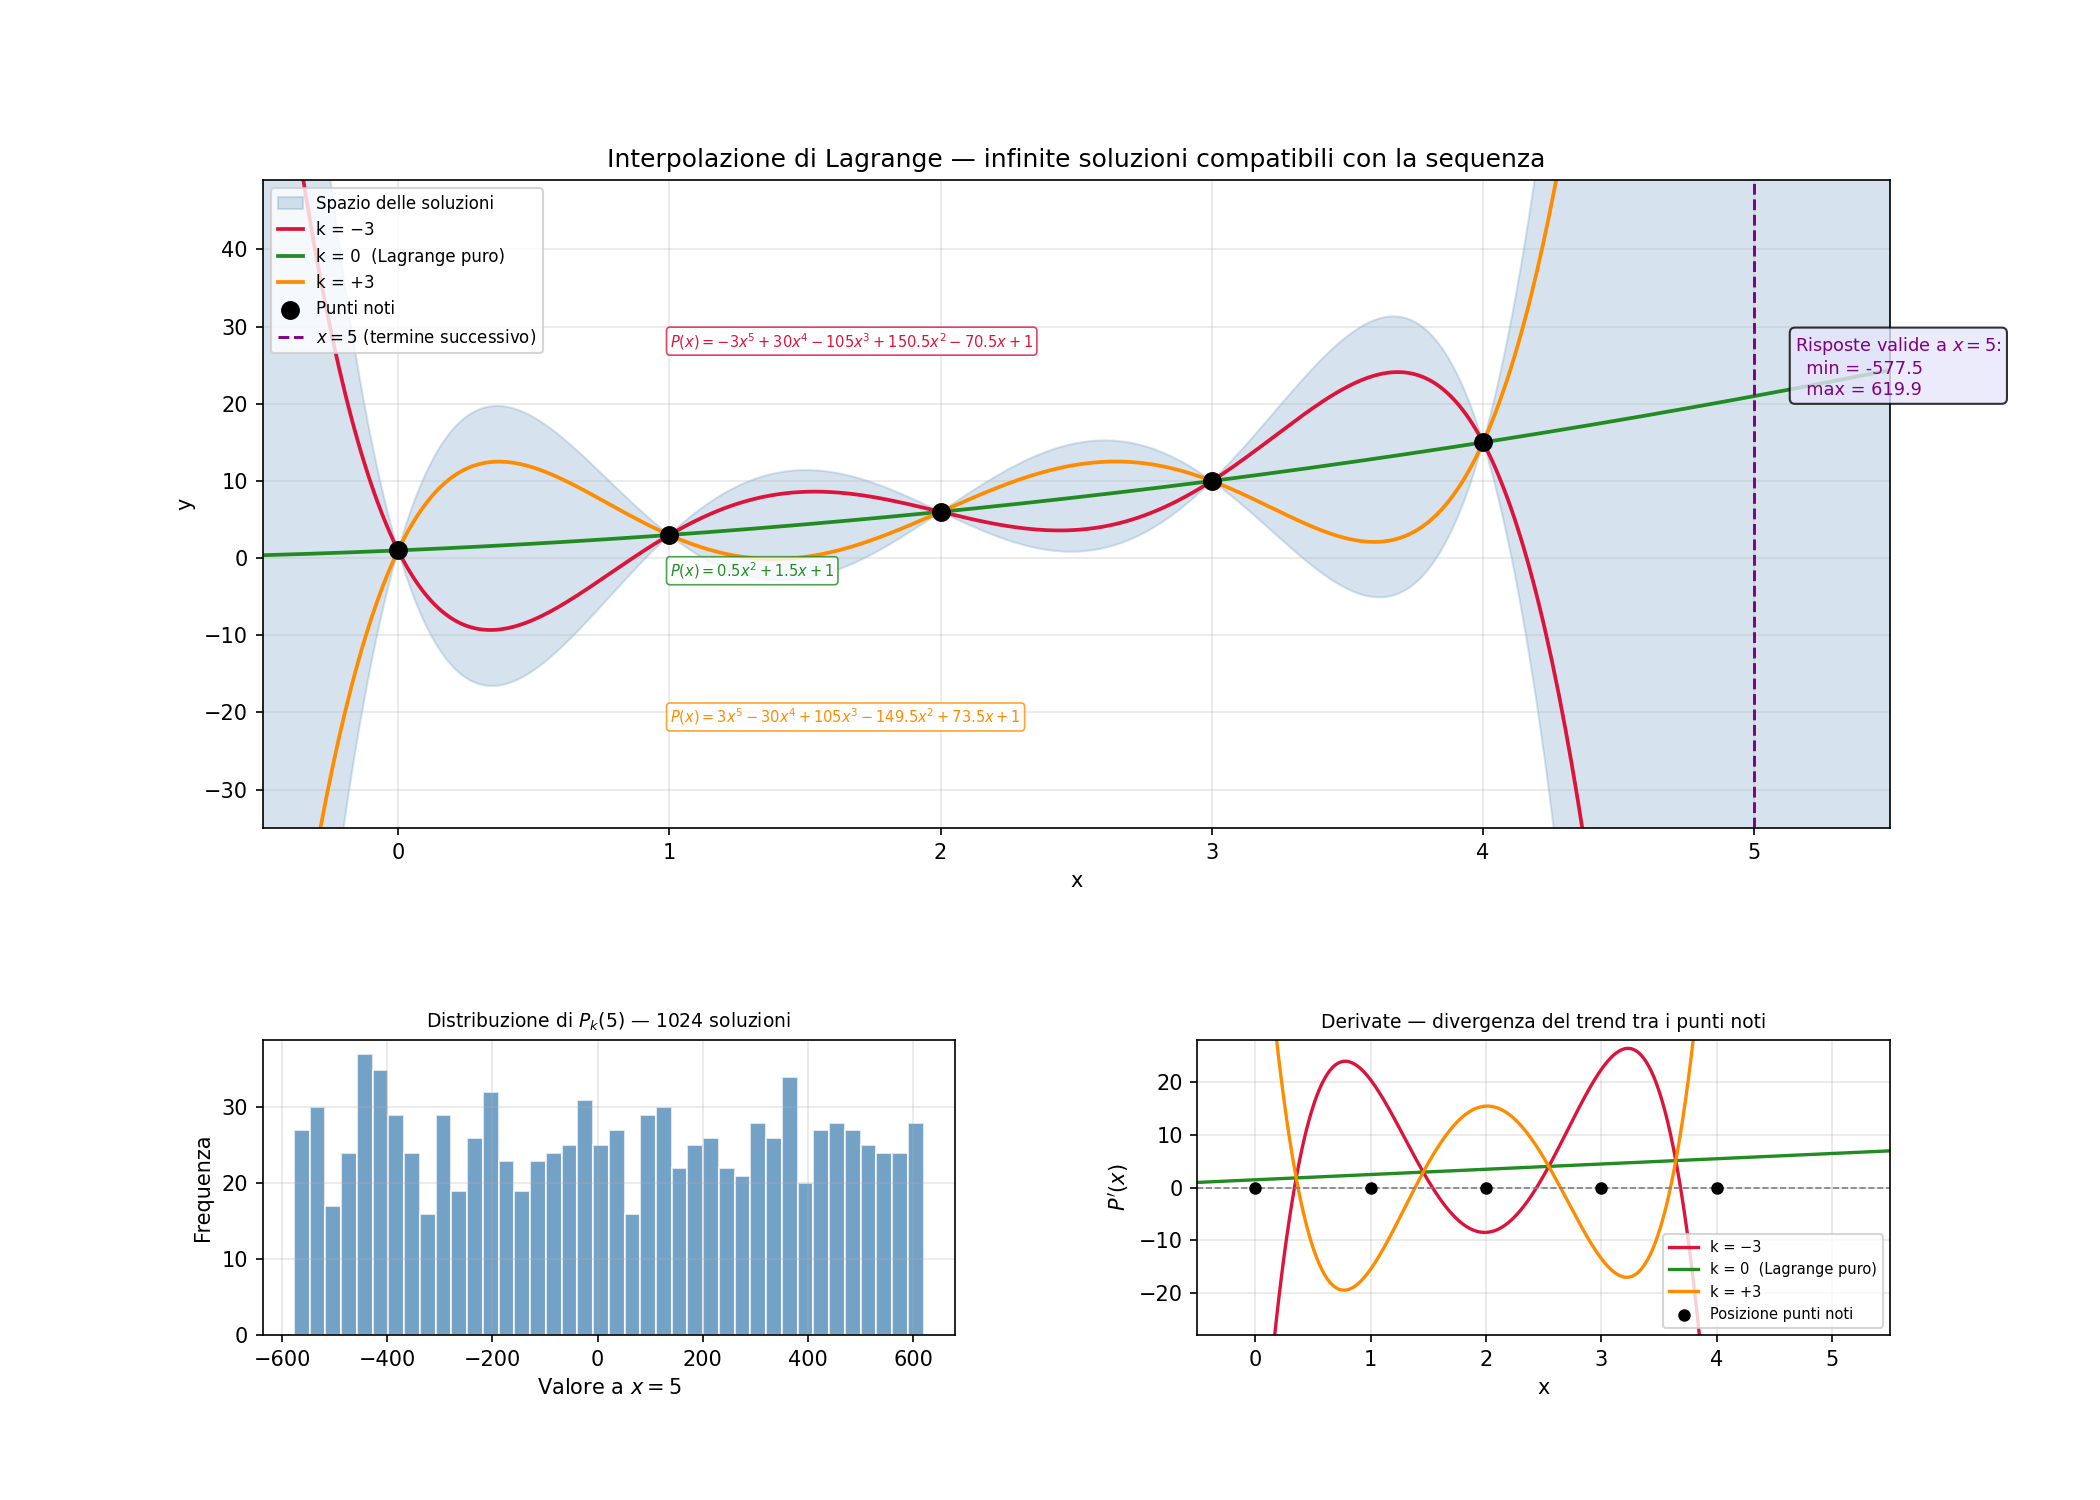
\includegraphics[width=\linewidth]{lagrange_plot.png}
    \caption{Visualization of the family of interpolants
    $P_k(x)=P(x)+kW(x)$ produced by the repository code. The blue region shows
    the envelope of the sampled solutions; the three colored curves show
    individual examples; the histogram illustrates the distribution of values
    obtainable at the next point; the derivative panel shows how sharply the
    behavior between observed points may diverge even when all curves coincide
    exactly on those points.}
    \label{fig:plot}
\end{figure}

The visual message of the figure is simple:
\begin{itemize}
    \item all curves pass through the same known points;
    \item between one observed point and the next, and especially beyond the
          last point, they may nevertheless diverge substantially;
    \item the value at the next point is not fixed by the data but depends on
          the additional parameter $k$.
\end{itemize}

The histogram of the value at $x=n$ is nearly uniform because, once the data are
fixed, the value
\[
P_k(n)=P(n)+kW(n)
\]
depends linearly on $k$. Sampling $k$ uniformly therefore also samples the
predicted value at the next point uniformly, up to the finite effects of
numerical sampling.

\section{What the \texorpdfstring{$g$}{g} Factor Is}
\label{sec:g}

\subsection{Historical origin of the idea}

The $g$ factor takes its name from the word \emph{general}. The idea goes back
to Spearman, who observed a robust empirical pattern: scores obtained by
different people on different cognitive tasks tend to be positively correlated
with one another~\cite{spearman1904}. Intuitively:

\begin{quote}
someone who performs relatively well on a verbal reasoning task tends, on
average, also to perform relatively well on numerical, spatial, or memory tasks,
even though clear differences in profile obviously remain.
\end{quote}

This regularity is often called the \emph{positive manifold}. It is one of the
most replicated findings in the psychometrics of intelligence~\cite{kovacs2016,
vandermaas2006}.

\subsection{An intuitive definition}

The $g$ factor is not a question, not a single task, and not a number read
directly from a psychological instrument. It is a \emph{latent factor}: a
variable not directly observed, introduced in order to explain the portion of
variance that many cognitive tests appear to share.

Stated even more simply:
\begin{quote}
$g$ is the name given to the common part that emerges when many different
cognitive tests ``move together'' in the data.
\end{quote}

This point is essential. The $g$ factor is a statistically constructed quantity
that receives a theoretical interpretation; it is not an object observed
directly.

\subsection{What g is \emph{not}}

To avoid confusion, a few distinctions are worth stating explicitly.

\begin{itemize}
    \item \textbf{$g$ is not identical to a raw IQ score.} An IQ score is
          usually a standardized index derived from a specific battery; $g$ is
          the latent common factor estimated from the relations among tasks.
    \item \textbf{$g$ does not exhaust every theory of intelligence.} There are
          hierarchical models, multifactor models, and alternative explanations
          of the positive manifold~\cite{cattell1963, carroll1993,
          sternberg1985, sternberg1999, kovacs2016, vandermaas2006}.
    \item \textbf{$g$ does not automatically imply a single simple cause.} Some
          authors interpret it as the index of a broad general capacity; others
          interpret it as an emergent product of partially overlapping cognitive
          processes~\cite{kovacs2016, vandermaas2006}.
\end{itemize}

\subsection{The relation between g, broad abilities, and specific abilities}

Contemporary psychometric literature often describes intelligence in hierarchical
terms. In models inspired by the work of Cattell, Horn, and Carroll, one may
distinguish at least three conceptual levels~\cite{cattell1963, carroll1993}:
\begin{enumerate}[label=\arabic*.]
    \item \textbf{specific abilities}: performance in narrowly defined tasks;
    \item \textbf{broad abilities}: for example fluid intelligence ($G_f$),
          crystallized intelligence ($G_c$), memory, or processing speed;
    \item \textbf{the general factor}: the common component that stands above
          multiple broad abilities.
\end{enumerate}

In this language, sequence items are usually interpreted as tasks that load
especially on abstract reasoning and rule induction, often close to what is
called fluid intelligence. But the fact that an item loads on $g$ does not mean
that its semantic content is irrelevant. This is exactly where the question of
construct validity arises.

\section{How the \texorpdfstring{$g$}{g} Factor Is Calculated}
\label{sec:gcalc}

\subsection{The general idea}

Saying that one ``calculates $g$'' can be misleading. In reality, $g$ is not
measured in the same way that temperature is measured with a thermometer. More
precisely:
\begin{enumerate}[label=\arabic*.]
    \item scores are collected from many people across many cognitive tests;
    \item the way those scores correlate is examined;
    \item a statistical model is estimated in order to summarize the shared part
          of the observed performance.
\end{enumerate}

The final result is an estimate of a common latent factor. That estimate always
depends, at least in part, on the chosen battery, the sample under study, and
the statistical method that is used.

\subsection{The stages of the calculation, explained without unnecessary jargon}

\begin{table*}[t]
    \centering
    \begin{tabular}{>{\raggedright\arraybackslash}p{1.8cm} >{\raggedright\arraybackslash}p{4.2cm} >{\raggedright\arraybackslash}p{7.2cm}}
        \toprule
        \textbf{Step} & \textbf{Operation} & \textbf{Intuitive meaning} \\
        \midrule
        1 & Administer a battery of different tests & One needs performance across non-identical tasks in order to see what they share. \\
        2 & Standardize the scores & Tests use different scales; standardization makes them comparable. \\
        3 & Build the correlation matrix & One measures how strongly results on different tests rise and fall together. \\
        4 & Extract the dominant common factor & One estimates the latent component that explains the largest share of shared covariation. \\
        5 & Estimate the \emph{loadings} & For each test, one assesses how strongly it depends on the general factor. \\
        6 & Compute individual \emph{factor scores} & For each person, one produces an estimate of their position on the general factor, given that battery and that method. \\
        \bottomrule
    \end{tabular}
    \caption{Intuitive outline of the estimation of the $g$ factor.}
    \label{tab:gsteps}
\end{table*}

\subsection{Step 1: collecting the scores}

Suppose we have $N$ people and $p$ cognitive tests. Let $x_{ij}$ denote the
score obtained by person $i$ on test $j$. The raw data therefore form an
$N \times p$ matrix.

Intuitively, each row is a person and each column is a task (vocabulary,
analogies, numerical series, mental rotation, memory, and so on).

\subsection{Step 2: standardization}

Different tests may use very different scales. One task may range from $0$ to
$20$, another from $200$ to $800$. To make them comparable, the scores are often
transformed into standardized scores:
\begin{equation}
z_{ij}=\frac{x_{ij}-\bar{x}_j}{s_j},
\label{eq:zscore}
\end{equation}
where $\bar{x}_j$ is the mean score on test $j$ and $s_j$ its standard
deviation.

Interpretation: $z_{ij}=0$ means ``average''; $z_{ij}=1$ means ``one standard
deviation above the mean''; $z_{ij}=-1$ means ``one standard deviation below the
mean''.

\subsection{Step 3: the correlation matrix}

Once the scores have been standardized, one computes the correlation matrix
\[
R=(r_{jk})_{j,k=1}^{p},
\]
where each coefficient $r_{jk}$ measures the degree of association between tests
$j$ and $k$.

If many coefficients are positive, one observes the positive manifold that
historically motivated the introduction of $g$~\cite{spearman1904}.

\subsection{Step 4: the factor model}

In a simplified one-factor version, the standardized score of person $i$ on test
$j$ is written as
\begin{equation}
z_{ij}=\lambda_j g_i + \epsilon_{ij}.
\label{eq:factor}
\end{equation}

Here:
\begin{itemize}
    \item $g_i$ is the latent position of person $i$ on the general factor;
    \item $\lambda_j$ is the loading of test $j$ on $g$;
    \item $\epsilon_{ij}$ contains what remains: test-specific variance,
          measurement error, and variability not explained by the common factor.
\end{itemize}

If $\lambda_j$ is large in absolute value, that test depends strongly on the
general factor. If it is small, the test reflects less $g$ and more task-specific
components.

In matrix form, the common-factor model can be summarized as
\begin{equation}
R \approx \Lambda\Lambda^\top + \Psi,
\label{eq:commonfactor}
\end{equation}
where $\Lambda$ contains the loadings and $\Psi$ the non-shared part.

\subsection{Step 5: extracting the factor}

Operationally, the model parameters must be estimated. Several procedures are
available:
\begin{itemize}
    \item exploratory factor analysis;
    \item confirmatory factor models;
    \item hierarchical or bifactor models.
\end{itemize}

All of these approaches try, in different ways, to summarize the covariation
among tests. The key point for the non-specialist reader is this:

\begin{quote}
the value of $g$ does not simply fall out of the data automatically; it emerges
from a statistical model chosen by the researcher.
\end{quote}

\subsection{Step 6: computing the individual factor score}

Once the loadings have been estimated, one may assign to each person an estimate
of their score on $g$, often denoted by $\hat{g}_i$. In schematic form:
\begin{equation}
\hat{g}_i = w_1 z_{i1} + w_2 z_{i2} + \cdots + w_p z_{ip},
\label{eq:factorscore}
\end{equation}
where the weights $w_1,\ldots,w_p$ depend on the scoring method used
(regression scoring, Bartlett scoring, and so on).

This point is often overlooked in popular discussions:
\begin{quote}
an individual $g$ score is a \emph{model-based estimate}, not a directly
observed quantity.
\end{quote}

\subsection{A purely illustrative mini-example}

Suppose a battery contains four tests: vocabulary, numerical series, mental
rotation, and working memory. After factor analysis, one might obtain
hypothetical loadings like those shown in Table~\ref{tab:loadings}.

\begin{table*}[t]
    \centering
    \begin{tabular}{lcc}
        \toprule
        \textbf{Test} & \textbf{Loading on $g$} & \textbf{Estimated shared variance ($\lambda^2$)} \\
        \midrule
        Vocabulary & 0.72 & 0.52 \\
        Numerical series & 0.78 & 0.61 \\
        Mental rotation & 0.69 & 0.48 \\
        Working memory & 0.64 & 0.41 \\
        \bottomrule
    \end{tabular}
    \caption{Illustrative example of factor loadings. The values are shown only
    for didactic purposes.}
    \label{tab:loadings}
\end{table*}

A person who obtains high standardized scores across several tasks will normally
receive a higher estimate of $\hat{g}$. But that estimate depends on the
weights, the loadings, and the battery. Changing the test or the method may
yield a non-identical estimate.

\subsection{Important distinction: first principal component versus g}

\begin{remark}
In practice one sometimes hears that $g$ is simply the first principal
component. That formulation is convenient but imprecise. PCA summarizes the
total variance of the observed scores; common factor analysis instead tries to
model the shared variance among tasks. The two outcomes may resemble each other,
but they are not conceptually the same thing.
\end{remark}

\section{What Follows for Construct Validity}
\label{sec:validity}

\subsection{First clarification: the critique does not say that tests ``measure nothing''}

This distinction is crucial. From the fact that a sequence item is
underdetermined, it does \emph{not} follow that every intelligence test is
useless or lacks predictive power. Indeed, the existence of the positive
manifold and the ability of some batteries to predict educational outcomes are
well documented~\cite{deary2007, jensen1998}.

The critique developed here is narrower:
\begin{quote}
even when a test is useful, the question remains whether it measures exactly the
construct it claims to measure and whether each of its items is interpreted in
the way it is ordinarily presented.
\end{quote}

\subsection{What construct validity is}

\begin{definition}[Construct validity]
A test has construct validity if the interpretation of its scores as measures of
a given theoretical construct is justified by evidence and by a coherent theory
of the process that produces the responses~\cite{cronbach1955, borsboom2004}.
\end{definition}

In intuitive terms, construct validity answers the question:
\begin{quote}
``when I observe this score, do I genuinely have good reasons to say that I am
measuring the psychological property the test claims to measure?''
\end{quote}

Good correlations with other tests or with certain external outcomes are
important, but they do not by themselves exhaust the problem of what the score
means.

\subsection{Where the underdetermination argument applies}

In the case of numerical completion items, the point is not that such items are
always bad items. The point is that their interpretation requires one more level
of precision.

If the observed sequence does not by itself determine a unique continuation,
then full credit awarded to one specific answer rewards at least one of the
following abilities:
\begin{enumerate}[label=\arabic*.]
    \item recognizing the pattern the test designer \emph{intended};
    \item applying an implicit criterion of simplicity or familiarity;
    \item accepting the framing of the question, namely the idea that there must
          be one expected continuation;
    \item working quickly within shared but unstated conventions.
\end{enumerate}

All of these abilities may be real and useful. But they do not automatically
coincide with ``general intelligence'' in the broadest philosophical sense of
the term.

\subsection{The role of the g factor in the standard defense}

The standard psychometric defense often runs as follows:
\begin{enumerate}[label=\arabic*.]
    \item scores on many cognitive items correlate positively;
    \item a general factor $g$ is extracted from that structure;
    \item an item that loads on $g$ is treated as a good indicator of general
          intelligence.
\end{enumerate}

This line of reasoning is not without force. But it does not settle the whole
issue. An item may load on $g$ and still reward more specific competences than
the term ``intelligence'' suggests.

\subsection{The circularity that should be avoided}

Precision matters here. It would be incorrect to say that the entire
psychometrics of $g$ is an empty tautology. It is not. There are real data,
replicated correlations, and relations with external outcomes. Nonetheless,
there is a \emph{partial circularity} that deserves attention:

\begin{itemize}
    \item items are selected in part because they show good correlations with
          other tests in the battery;
    \item the factor $g$ is estimated from batteries constructed in that way;
    \item the fact that an item loads on $g$ says a great deal about its
          coherence with the battery, but by itself it does not fully answer the
          question of what cognitive content the item actually rewards.
\end{itemize}

In other words, \emph{a high loading on $g$} and \emph{clarity of construct}
are not synonyms.

\subsection{What a sequence item plausibly measures}

In light of the preceding discussion, a more careful and more precise
formulation might be the following:

\begin{quote}
sequence items measure, at least in part, the ability to infer a conventional
rule judged appropriate by the testing context, under time constraints and with
incomplete information.
\end{quote}

This formulation is less sweeping than ``it measures intelligence in general'',
but it is probably closer to what the observed behavior actually supports.

\section{Comparison with Broader Perspectives on Intelligence}
\label{sec:broader}

Critiques of reducing intelligence to a single index are not new. Sternberg
argued, in different forms, that traditional tests capture only part of the
abilities that matter and that one must also consider creative, practical, and
meta-cognitive components~\cite{sternberg1985, sternberg1999}. Stanovich argued
that intelligence tests, even when useful, leave out dispositions that are
central to rational judgment, evidence evaluation, and sound everyday reasoning~\cite{stanovich2009}.

This literature does not by itself prove the mathematical thesis of the present
paper, but it situates it within a broader framework: a test may be empirically
useful and still incomplete with respect to what many people ordinarily mean by
the word ``intelligence''.

Sequence items are especially instructive because they display, in concentrated
form, the gap between:
\begin{itemize}
    \item a well-defined performance within a testing convention;
    \item the more ambitious claim of measuring a general capacity for
          reasoning.
\end{itemize}

\section{Limits of the Argument}
\label{sec:limits}

A rigorous paper should state not only what it shows, but also what it does not
show. The main limits are four.

\begin{enumerate}[label=\arabic*.]
    \item \textbf{Not all test items are equally ambiguous.}
          Some problems include contextual clues or implicit constraints strong
          enough to reduce the space of reasonable interpretations.

    \item \textbf{Mathematical underdetermination does not cancel practical
          usefulness.} In many real settings it may be entirely useful to test
          whether a person can quickly recognize simple, conventional patterns.

    \item \textbf{A single item is not the same as the whole battery.}
          Psychometric batteries aggregate many tasks precisely in order to
          reduce random error and increase overall reliability.

    \item \textbf{The argument primarily targets interpretation of the
          construct.} Its main target is not the mere existence of correlations
          or predictive validity, but the conceptual leap from those facts to
          the claim that one numerical answer is the only logically correct one
          and that recognizing it straightforwardly coincides with general
          intelligence.
\end{enumerate}

\section{Conclusions}
\label{sec:conclusion}

The central thesis of the article can be summarized in one sentence:
\begin{quote}
a finite sequence, taken by itself, does not uniquely determine the next term;
to obtain a unique answer, one must introduce additional constraints or
conventions.
\end{quote}

The Lagrange interpolation theorem and the construction of the family
$P(x)+W(x)H(x)$ make it possible to establish this point in a simple, formal,
and highly general way. From this it does not follow that intelligence tests
are worthless; it does follow that the interpretation of their sequence items
must be more sober and more precise.

When correctly understood, the $g$ factor is a latent factor extracted from the
correlational structure among cognitive tests. It is a powerful and historically
central statistical tool in psychometrics. But the fact that an item loads on
$g$ is not, by itself, enough to settle every question about what that item
means. Construct validity also requires an analysis of the cognitive process the
item rewards.

In the case of numerical completion items, the most defensible conclusion is
therefore the following: they certainly measure something, but that something is
better described as the ability to infer and apply a conventionally expected
rule within a testing context than as direct and unproblematic access to
intelligence in a fully general sense.

A more transparent design could improve this situation in at least two ways:
\begin{enumerate}[label=\arabic*.]
    \item by explicitly stating the admissible class of rules;
    \item by rewarding not only the final answer but also the quality of the
          justification and the ability to recognize when a problem is
          underconstrained.
\end{enumerate}

\appendix

\section{Essential Glossary}
\label{sec:glossary}

\begin{description}[style=nextline, leftmargin=2.7cm]
    \item[Interpolation]
    The construction of a function that passes exactly through a given set of
    data points.

    \item[Underdetermination]
    A situation in which the available data are insufficient to select a unique
    solution without further assumptions.

    \item[Parsimony]
    A preference for simpler explanations or models, all else being equal.

    \item[Correlation]
    A measure of the extent to which two variables tend to rise or fall
    together.

    \item[Latent variable]
    A theoretical variable not directly observed, introduced to explain
    regularities in observed data.

    \item[Factor loading]
    A coefficient indicating how strongly a test is associated with a latent
    factor.

    \item[Factor score]
    A numerical estimate, for an individual, of that person's position on a
    latent factor.

    \item[Construct validity]
    The theoretical and empirical justification for interpreting a score as a
    measure of a given psychological property.
\end{description}

\section*{Technical Appendix on the Repository}
\addcontentsline{toc}{section}{Technical Appendix on the Repository}

The repository includes a computational demonstration consistent with the
mathematical thesis of the paper:
\begin{itemize}
    \item \texttt{lagrange.cu} computes the family of perturbed polynomials in
          parallel;
    \item \texttt{output.csv} contains the numerical envelope of the solutions;
    \item \texttt{plot.py} constructs the final figure;
    \item \texttt{lagrange\_plot.png} visualizes the result.
\end{itemize}

This empirical component does not replace the theoretical argument, but it has
important pedagogical value: it makes visible, at a glance, how wide the family
of solutions compatible with the same observed points can be.

\begin{thebibliography}{99}

\bibitem{spearman1904}
Spearman, C. (1904).
``General Intelligence,'' Objectively Determined and Measured.
\textit{The American Journal of Psychology}, 15(2), 201--293.
doi:10.2307/1412107

\bibitem{cronbach1955}
Cronbach, L.~J., \& Meehl, P.~E. (1955).
Construct validity in psychological tests.
\textit{Psychological Bulletin}, 52(4), 281--302.
doi:10.1037/h0040957

\bibitem{cattell1963}
Cattell, R.~B. (1963).
Theory of fluid and crystallized intelligence: A critical experiment.
\textit{Journal of Educational Psychology}, 54(1), 1--22.
doi:10.1037/h0046743

\bibitem{carroll1993}
Carroll, J.~B. (1993).
\textit{Human Cognitive Abilities: A Survey of Factor-Analytic Studies}.
Cambridge University Press.
doi:10.1017/CBO9780511571312

\bibitem{jensen1998}
Jensen, A.~R. (1998).
\textit{The g Factor: The Science of Mental Ability}.
Greenwood Publishing.

\bibitem{sternberg1985}
Sternberg, R.~J. (1985).
\textit{Beyond IQ: A Triarchic Theory of Human Intelligence}.
Cambridge University Press.

\bibitem{sternberg1999}
Sternberg, R.~J. (1999).
The theory of successful intelligence.
\textit{Review of General Psychology}, 3(4), 292--316.
doi:10.1037/1089-2680.3.4.292

\bibitem{borsboom2004}
Borsboom, D., Mellenbergh, G.~J., \& van Heerden, J. (2004).
The concept of validity.
\textit{Psychological Review}, 111(4), 1061--1071.
doi:10.1037/0033-295X.111.4.1061

\bibitem{vandermaas2006}
van der Maas, H.~L.~J., Dolan, C.~V., Grasman, R.~P.~P.~P., Wicherts, J.~M.,
Huizenga, H.~M., \& Raijmakers, M.~E.~J. (2006).
A dynamical model of general intelligence: The positive manifold of intelligence
by mutualism.
\textit{Psychological Review}, 113(4), 842--861.
doi:10.1037/0033-295X.113.4.842

\bibitem{deary2007}
Deary, I.~J., Strand, S., Smith, P., \& Fernandes, C. (2007).
Intelligence and educational achievement.
\textit{Intelligence}, 35(1), 13--21.
doi:10.1016/j.intell.2006.02.001

\bibitem{stanovich2009}
Stanovich, K.~E. (2009).
\textit{What Intelligence Tests Miss: The Psychology of Rational Thought}.
Yale University Press.

\bibitem{kovacs2016}
Kovacs, K., \& Conway, A.~R.~A. (2016).
Process overlap theory: A unified account of the general factor of intelligence.
\textit{Psychological Inquiry}, 27(3), 151--177.
doi:10.1080/1047840X.2016.1153946

\bibitem{taleb2019}
Taleb, N.~N. (2019).
\textit{IQ is largely a pseudoscientific swindle}.
Medium. \url{https://medium.com/incerto/iq-is-largely-a-pseudoscientific-swindle-f131c101ba39}

\bibitem{gould1981}
Gould, S.~J. (1981).
\textit{The Mismeasure of Man}.
W.~W. Norton \& Company.

\bibitem{gardner1983}
Gardner, H. (1983).
\textit{Frames of Mind: The Theory of Multiple Intelligences}.
Basic Books.

\bibitem{knill2014}
Knill, O. (2014).
\textit{Math 1a — Sequences and IQ tests}.
Harvard University, course notes.

\end{thebibliography}

\end{document}
